\chapter{Architectuur}\label{ch:Architectuur}
Om bruikbare informatie te kunnen tonen aan de gebruiker moet de informatie welke door de Software Composition Analysis(SCA) Tool wordt geleverd worden bewerkt naar een datamodel waarbij alleen de informatie die relevant is om te tonen wordt opgeslagen. Daarnaast moet het systeem in staat zijn om periodiek een analyse uit te voeren op projecten die bekend zijn binnen de module. In figuur~\ref{fig:SOUP-Components} is te zien hoe onderdelen met elkaar in verbinden staan.
In de secties hieronder wordt ieder onderdeel ver uitgwerkt op een architectonisch niveau.

\begin{figure}[bth]
    \myfloatalign
    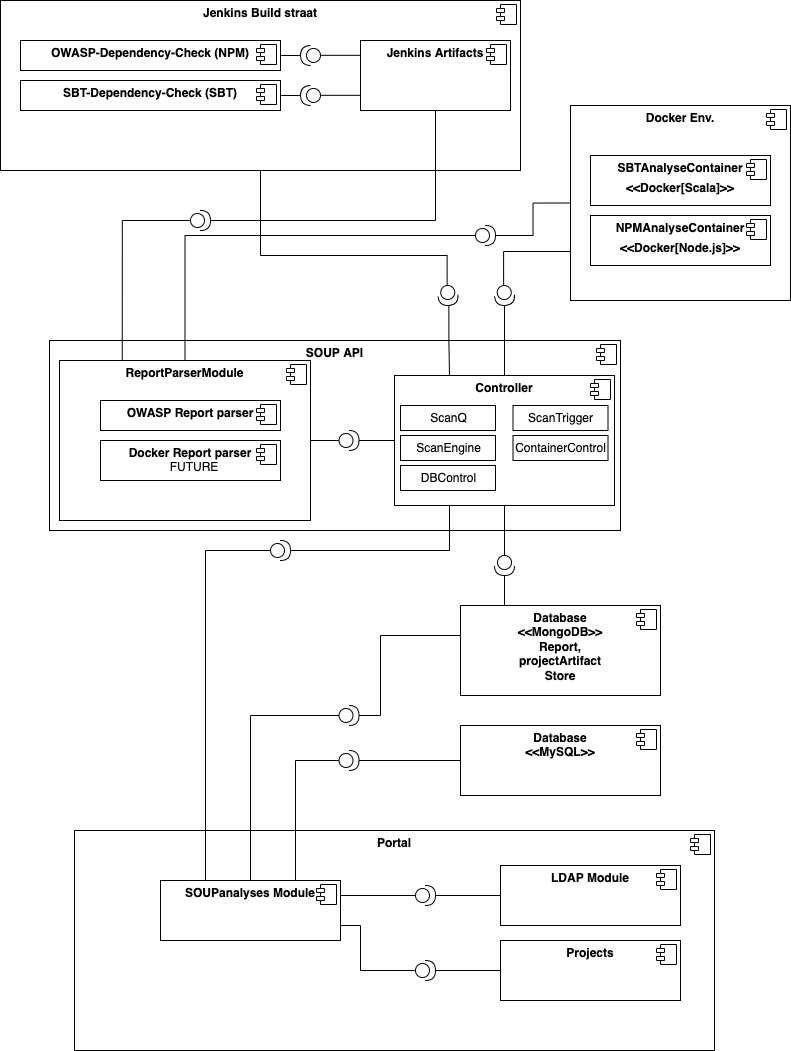
\includegraphics[width=9cm]{gfx/UMLcomponentDiagram}
    \caption{Componenten SOUP Analyse Systeem}
    \label{fig:SOUP-Components}
\end{figure}


\section{SOUPAPI}\label{sec:soupapi}
De SOUP API staat centraal in het nieuwe systeem en is verantwoordelijk voor de verwerking van de informatie uit de SCA tooling te halen. Een andere taak is het faciliteren van een systeem dat verantwoordelijk is voor het periodiek scannen van de door de module bekende projecten.

Voor de verwerking van informatie is de ReportParser verantwoordelijk  Het wordt in gezet voor het vertalen en omzetten van de data uit rapporten die door de SCA Tooling worden gegenereerd naar data die gebruikt worden binnen de SOUP module van de portal. In dit ontwerp is er een parser aanwezig voor het vertalen van de OWASP-engine rapporten\footnote{De SCA tooling in het vorige hoofdstuk genereren beide rapporten in het zelfde JSON schema}. In de toekomst zullen er meerdere parsers moeten worden toegevoegd op het moment dat er een andere runtime wordt meegenomen welke niet door de OWASP engine kunnen worden gescanned.

De Controller is verantwoordelijk voor de taken die te maken hebben met het periodiek scannen van projecten Het heeft faciliteiten zoals een scanQ waarin de projecten staan die gescanned moeten worden. Een analyser die op het moment dat een project aan de beurt is om geanalyseerd te worden een aantal subtaken sequentieel uitvert per module binnen een project.
In grote lijnen wordt er een dockercontainer opgezet per module waarin alle benodigde bestanden (dependency declaraties en dergelijke) worden geplaats. Vervolgens een analyse wordt uitbgevoer waaruit de resultaten naar de ReportParser kan worden gestuurt voor analyse. De exacte werking wpordt verderop in het document technisch uitgewerkt.

\section{Jenkins buildtstraat}



\section{Jenkins Buildstraat}


\section{Portal}